\DeclareSymbolFont{AMSb}{U}{msb}{m}{n}
\documentclass[11pt,noamsfonts]{amsart}
\usepackage[left=1.5in, right=1.5in, top=1.2in, bottom=1.2in]{geometry}
\usepackage{mathtools}
\usepackage{braket}
\usepackage{enumitem}
\usepackage[charter,expert]{mathdesign}
\usepackage[scaled=.96,osf]{XCharter}% matches the size used in math
\usepackage[tracking]{microtype}
\usepackage{tikz-cd}
\usepackage{stmaryrd}
\usepackage{comment}
\usepackage[scr=esstix]{mathalfa}

\usepackage{caption}
\usepackage{subcaption}

\usepackage{hyperref}
\linespread{1.04}

\usepackage{enumitem}
\setlist[1]{labelindent=\parindent}
\setlist[enumerate]{labelsep=0.5em}
\setlist[enumerate,1]{label={\upshape (\roman*)}, ref={\upshape (\roman*)}}
\setlist[itemize]{label={--}}

\DeclareMathOperator{\Sym}{Sym}

\makeatletter
\let\c@equation\c@section
\let\theequation\thesection
\makeatother

%found on https://tex.stackexchange.com/a/565122 with improvements from TikZ manual:
\tikzset{>={Straight Barb[length=2pt,width=4pt]}, commutative diagrams/arrow style=tikz}

\usepackage[utf8]{inputenc}

\newcommand{\todo}[1]{\footnote{{\sc\color{red}Todo.} #1}}

% Point Formats
\newcommand{\pointheader}{\vspace{2mm}\noindent\refstepcounter{section}\textbf{\thesection.}}
\newcommand{\point}{\pointheader~}
\newcommand{\tpoint}[1]{\pointheader~{\bf #1. ---}}
\newcommand{\epoint}[1]{\pointheader~{\em #1.}}
\newcommand{\bpoint}[1]{\pointheader~{\bf #1.}}

% QED Symbol
\newcommand{\psqedsymb}{\(\blacksquare\)}
\renewcommand{\qed}{~\hfill{\psqedsymb}}


\makeatletter
\newcommand*{\coloneqq}{\mathrel{\rlap{%
           \raisebox{0.3ex}{$\m@th\cdot$}}%
           \raisebox{-0.3ex}{$\m@th\cdot$}}%
           =}
\newcommand{\eqqcolon}{=%
           \mathrel{\rlap{%
           \raisebox{0.3ex}{$\m@th\cdot$}}%
           \raisebox{-0.3ex}{$\m@th\cdot$}}}
\makeatother

\DeclareMathOperator{\Hom}{Hom}

% Taken from the same Stack Overflow latex-function-diagram as below
\usepackage{tikz}
\usepackage{graphicx}
\usepackage{pgf,pgfplots}
\usetikzlibrary{math,arrows,positioning,shapes,fit,calc}

% Taken from the Overleaf example
\usepackage{hyperref}
\hypersetup{
    colorlinks=true,
    linkcolor=blue,
    filecolor=magenta,      
    urlcolor=cyan,
    pdftitle={Overleaf Example},
    pdfpagemode=FullScreen,
    }

\urlstyle{same}

\title{Crude motivation of Temperley-Lieb monoid}
\begin{document}
\maketitle

(This whole story is mostly taken from \url{http://people.mpim-bonn.mpg.de/geordie/BMW.pdf})

There's a standard depiction of a finite set, possibly referencing Venn diagrams,
as a collection of dots, possibly labeled with letters, possibly circled or surrounded by a smooth line of some sort.

% taken from https://tex.stackexchange.com/questions/538039/latex-function-diagram
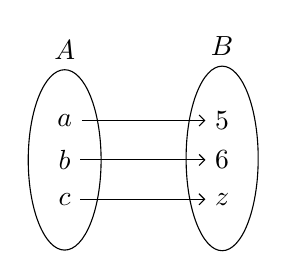
\begin{tikzpicture}
    \foreach[count=\i] \lseti/\lsetmi in {{A}/{$a$,$b$,$c$},{B}/{5,6,$z$}} {
        \begin{scope}[local bounding box=\lseti, x=2cm, y=0.5cm]
        \foreach[count=\j] \lj in \lsetmi {
            \node[minimum width=1em] (n-\j-\lseti) at (\i,-\j) {\lj};
        }
        \end{scope}
        \node[ellipse, draw, fit=(\lseti), label={above:$\lseti$}] {};
    }
    \draw[->] (n-1-A) -- (n-1-B);
    \draw[->] (n-2-A) -- (n-2-B);
    \draw[->] (n-3-A) -- (n-3-B);
\end{tikzpicture}

There's a standard depiction of a particular function from a finite set to another finite set, which leans on and extends that depiction of a finite set:
\begin{itemize}
\item The source finite set is depicted as a collection of dots, possibly labeled with letters,
possibly circled or surrounded by a smooth line of some sort.
\item The target finite set is also depicted similarly.
\item The association of an element in the source to its image in the target is a line.
\end{itemize}

One purpose of this depiction is that it is relatively easy to overlap the depictions of
a pair of functions and obtain a depiction of their composition. Associativity of function composition is perhaps possible to `see' directly.

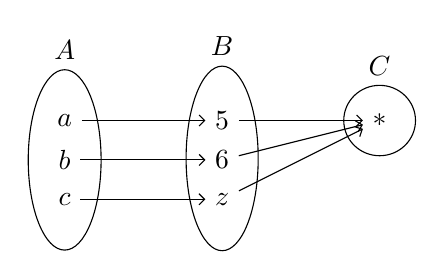
\begin{tikzpicture}
    \foreach[count=\i] \lseti/\lsetmi in {{A}/{$a$,$b$,$c$},{B}/{5,6,$z$},{C}/{$*$}} {
        \begin{scope}[local bounding box=\lseti, x=2cm, y=0.5cm]
        \foreach[count=\j] \lj in \lsetmi {
            \node[minimum width=1em] (n-\j-\lseti) at (\i,-\j) {\lj};
        }
        \end{scope}
        \node[ellipse, draw, fit=(\lseti), label={above:$\lseti$}] {};
    }
    \draw[->] (n-1-A) -- (n-1-B);
    \draw[->] (n-2-A) -- (n-2-B);
    \draw[->] (n-3-A) -- (n-3-B);

    \draw[->] (n-1-B) -- (n-1-C);
    \draw[->] (n-2-B) -- (n-1-C);
    \draw[->] (n-3-B) -- (n-1-C);
\end{tikzpicture}

Leaning on that depiction of a function, there is a relatively standard depiction of an element of the symmetric group on \(n\) elements, which uses two visually distinct, but parallel, depictions of what is conceptually the same finite set with \(n\) elements. Then the multiplication operation of the symmetric group is captured by the composition procedure above.

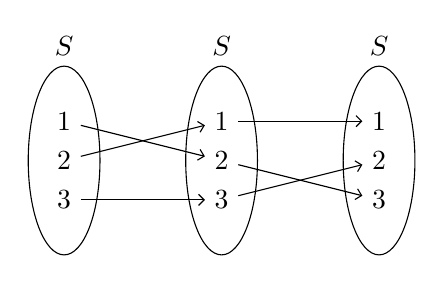
\begin{tikzpicture}
    \foreach[count=\i] \lseti/\lsetmi in {{S}/{1,2,3},{S}/{1,2,3},{S}/{1,2,3}} {
        \begin{scope}[local bounding box=\lseti, x=2cm, y=0.5cm]
        \foreach[count=\j] \lj in \lsetmi {
            \node[minimum width=1em] (n-\i-\j) at (\i,-\j) {\lj};
        }
        \end{scope}
        \node[ellipse, draw, fit=(\lseti), label={above:$\lseti$}] {};
    }
    \draw[->] (n-1-1) -- (n-2-2);
    \draw[->] (n-1-2) -- (n-2-1);
    \draw[->] (n-1-3) -- (n-2-3);

    \draw[->] (n-2-1) -- (n-3-1);
    \draw[->] (n-2-2) -- (n-3-3);
    \draw[->] (n-2-3) -- (n-3-2);

\end{tikzpicture}

\bpoint{The Brauer monoid}

There's a generalization of this ``multiply by drawing'' procedure, which is called the Brauer monoid.

The idea here is that we take an arbitrary pairing of the \(2 n\) dots (the \(n\) source dots and the \(n\) target dots) - so two ``source'' dots can be connected to each other, or two target dots can be connected to one another. So there's a natural injection; each element of the symmetric group on \(n\) elements can be found inside the elements of the Brauer monoid, and the Brauer monoid multiplication is equal to group multiplication on that submonoid.

There's a thing that can happen when you connect two of these together - you can get one of the original kind of diagrams, plus also some loops or bubbles. The nice thing to do with these seems to be to keep count of how many loops or bubbles an element has - so an arbitrary element of the Brauer monoid is actually one of these perfect matchings on \(2 n\) elements, plus a count of how many loops or bubbles it is supposed to have. Then the procedure for multiplication is the graphical one, plus you add the counts of how many loops or bubbles each side contributed, plus any new loops or bubbles created by the graphical multiplication, to get a new element of the Brauer monoid.

\bpoint{The Temperley-Lieb monoid}

There's another generalization of the original `multiply by drawing' procedure,
where you consider the arrows to be strands that can go over or under one another; this is the braid group.

The Temperley-Lieb monoid takes in some sense an opposite tactic to crossings from the braid group; it forbids them. The nice thing about this is that when you graphically multiply two crossing-free diagrams, then you obtain a crossing-free diagram, and so this is a moderately natural closed submonoid of the Brauer monoid - just like the symmetric group.

\bpoint{What do you do with them?}

I think one of the things that you try to do is to get from the diagrams to an alternative,
more crisp, algebraic, or formal way of calculating and proving with them. You do some arguing for a particular symbolic notation, some generators, some relations, using the diagrams, and then when you build something on top of that, you can use your notation, and only revisit the diagrams for motivation and intuition purposes.

I think another thing that you try to do is to follow along, in parallel, the mathematical traditions around the symmetric group. Representation theory looks at the ways that you can represent elements of a group by matrices - is there something corresponding in the Brauer, Braid, or Temperley-Lieb worlds?

TODO: more of this

\end{document}


\end{document}
